\section{Measurement Setup}
\label{sec:measurement-setup}

Experiments were performed on a QPU comprising 11 uncoupled superconducting
qubits hosted in a dilution refrigerator.  Control and readout were implemented
with a Quantum Machines OPX1000 equipped with a microwave front-end module
(MW-FEM), together with external cryogenic attenuators, filters, circulators,
and amplifiers.

A schematic of the setup is shown in Fig.~\ref{fig:diagram}.  The MW-FEM uses
direct digital synthesis and digital upconversion: a programmed complex pulse
envelope is translated to the configured microwave carrier and emitted directly
from an RF output, without an external analog local oscillator or IQ mixer
\cite{qm_opx1000_mwfem}.  For acquisition, the returned microwave signal is
digitally downconverted to a complex baseband stream.  QUA demodulation then
applies cosine and sine integration weights to the sampled signal and accumulates
the result to obtain the measured quadratures \cite{qm_opx_demodulation}.  Thus,
separate MW-FEM outputs provide the qubit-drive and resonator-readout tones,
while an MW-FEM input acquires the returning readout signal.  A dedicated DC
bias line was available but was not used in these measurements; consequently,
the qubits were not necessarily operated at their flux sweet spots.

The device was mounted at the mixing-chamber stage ($\sim$9 mK), with the drive
and readout lines attenuated across the refrigerator stages.  The returning
readout signal passed through circulators and a 4 K high-electron-mobility
transistor (HEMT) amplifier before entering the MW-FEM for digital
downconversion and demodulation.


\begin{figure}
    \centering
    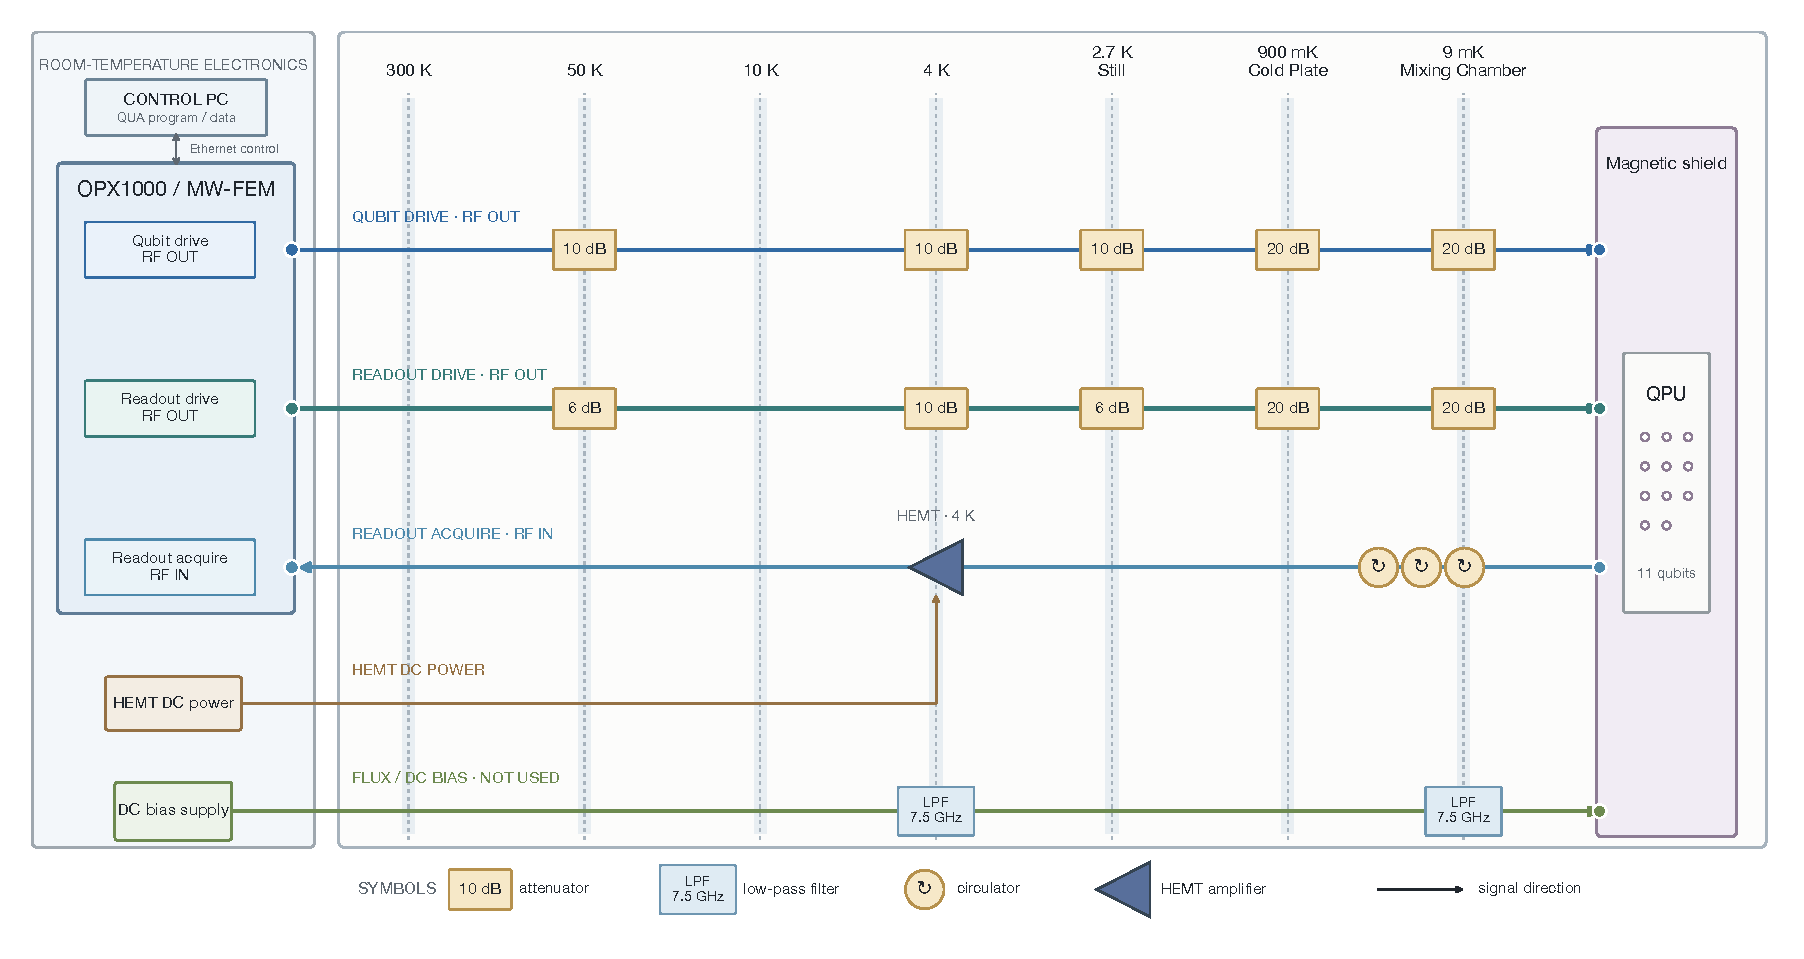
\includegraphics[width=0.98\linewidth]{figures/cryogenic_measurement_chain.pdf}
    \caption{Schematic of the experimental setup for qubit control and readout.
A control computer submits QUA programs and receives data over Ethernet.  The
OPX1000 MW-FEM directly generates the qubit-drive and resonator-readout RF
signals and acquires the returning readout signal.  Input lines are attenuated
across the 300 K, 50 K, 10 K, 4 K, still, cold-plate, and mixing-chamber stages.
The low-pass-filtered DC-bias line is shown for completeness but was not used.
At the mixing chamber, the device is isolated by circulators; the returning
readout signal is amplified by a 4 K HEMT before entering the MW-FEM for digital
downconversion and demodulation.}
    \label{fig:diagram}
\end{figure}

\subsection{Qubit coherence characterization}
\label{subsec:q1-coherence-characterization}

The energy-relaxation and Ramsey-dephasing times of the qubit used for the
spectroscopy measurements were characterized independently.  Figure~\ref{fig:q1-t1-t2}
shows representative measurements for qubit q1.  Fitting the excited-state
population to an exponential decay with a constant offset gives
$T_1=\MeasuredTOne~\mu\mathrm{s}$.  Fitting the positive-detuning Ramsey trace
to an exponentially damped sinusoid gives
$T_2^*=\MeasuredTTwoStar~\mu\mathrm{s}$.  The quoted uncertainties are
one-standard-deviation estimates obtained from the fit covariance matrices.
No associated Hahn-echo trace is available, so no measured Hahn-echo $T_2$ is
reported.  When one transverse time is required, we conservatively use
$T_{2,\mathrm{eff}}=T_2^*=\EffectiveTTwo~\mu\mathrm{s}$.  With the measured
$T_1$, this gives $T_\phi=\EffectiveTPhi~\mu\mathrm{s}$ through
$T_{2,\mathrm{eff}}^{-1}=(2T_1)^{-1}+T_\phi^{-1}$; this is not Hahn-echo
evidence.

\clearpage
\begin{figure}[t]
    \centering
    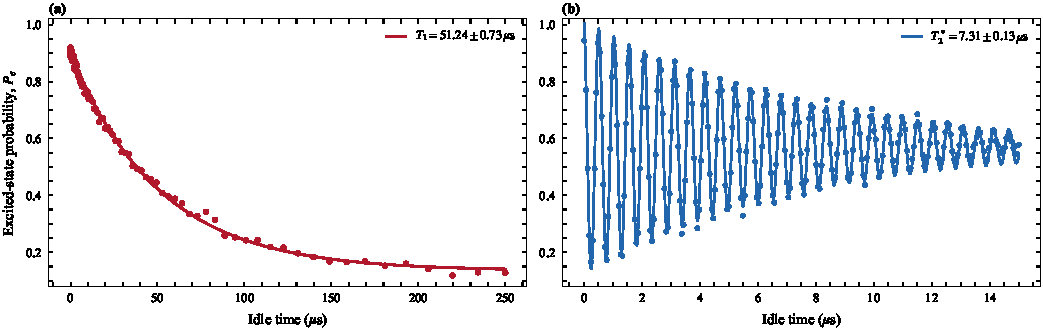
\includegraphics[width=\linewidth]{../figures/paper/05_q1_t1_t2.pdf}
    \caption{Independent coherence characterization of qubit q1.
    (a) Energy relaxation following state preparation, together with an
    exponential fit. (b) Ramsey fringes acquired with a positive
    $2~\mathrm{MHz}$ programmed detuning, together with an exponentially damped
    sinusoidal fit.}
    \label{fig:q1-t1-t2}
\end{figure}

\FloatBarrier
